\documentclass[12pt,letterpapper]{article}
\usepackage{newcent}
\usepackage[spanish]{babel}
\usepackage[utf8]{inputenc}
\usepackage[right=2cm,left=3cm,top=2cm,bottom=2cm,headsep=0cm]{geometry}

\usepackage{pdfpages}


\begin{document}
\author{Jesús Rodríguez Heras}
\title{Práctica 2 del tema 5}
\maketitle


Antes de realizar el diseño en logisim hay que realizar los cálculos correspondientes:

\section{Chips de memoria:}
\paragraph{1. ¿Cuántas direcciones tienen los chips de memoria proporcionados?\\} 
Cada chip tiene 8 Kilobytes de memoria, lo que pasado a bits son: $2^{16}$ bits. Si lo dividimos entre la unidad mínima direccionable por cada chip de memoria (4 bits), resultará el número de direcciones:
\begin{center}
	$\frac{2^{16}}{2^2}=2^{14}$
\end{center} 
Donde podemos ver que el número de direcciones de los chips es $2^{14}=16384$.

\paragraph{2. ¿Cuántos bits se necesitan para acceder a un dato de estos chips?\\}
El número de bits necesario para acceder a un dato es el exponente de la potencia calculada anteriormente, por lo tanto, se necesitan 14 bits.\\

\section{Memoria a diseñar:}
\paragraph{1. ¿Cuántos bits tendrá el bus de direcciones?\\}
Para averiguarlo, hacemos el mismo cálculo que en el primer apartado de los chips de memoria pero con los datos de la memoria a diseñar:
\begin{center}
	$\frac{96 \cdot 2^{13}}{2^4}\simeq2^{16}$
\end{center}
De donde se deduce que habrá 16 bits en el bus de direcciones.
\newpage
\paragraph{2. ¿Cuántos chips necesitaremos para formar la memoria?\\}
Dado que la memoria tiene un total de 96 Kilobytes y cada chip tiene una memoria de 8 Kilobytes, tenemos:
\begin{center}
	$\frac{96}{8}=12$
\end{center}
Lo que es igual a 12 chips de memoria.
\paragraph{3. Después de enviar una palabra a memoria...¿Cuántos chips se verán afectados?\\}
Debido a que la palabra está formada por 16 bits y la unidad mínima direccionable por los chips es de 4 bits, tenemos:
\begin{center}
	$\frac{16}{4}=4$
\end{center}
Por lo cual, se verán afectados 4 chips, lo que significa que los módulos de RAM deberán estar formados por 4 chips cada uno. Lo que a su vez significa que tenemos tres módulos de RAM de 4 chips cada uno.
\paragraph{4. ¿Se puede ampliar la memoria sin ampliar el número de bits en el bus de direcciones? Razona la respuesta.\\}
La diferencia entre los bits del bus de direcciones y los bits de direccionamiento de la memoria es de dos bits, lo que implica que habrá dos bits de direccionamiento.\\
Tenemos tres módulos de RAM y la capacidad de direccionar hasta un máximo de 4 módulos (debido a que hay dos bits de direccionamiento), por lo tanto, podemos añadir un módulo más (4 chips) sin alterar el número de bits del bus de direcciones.
\newpage

\section{Mapa de memoria:}
\begin{center}
	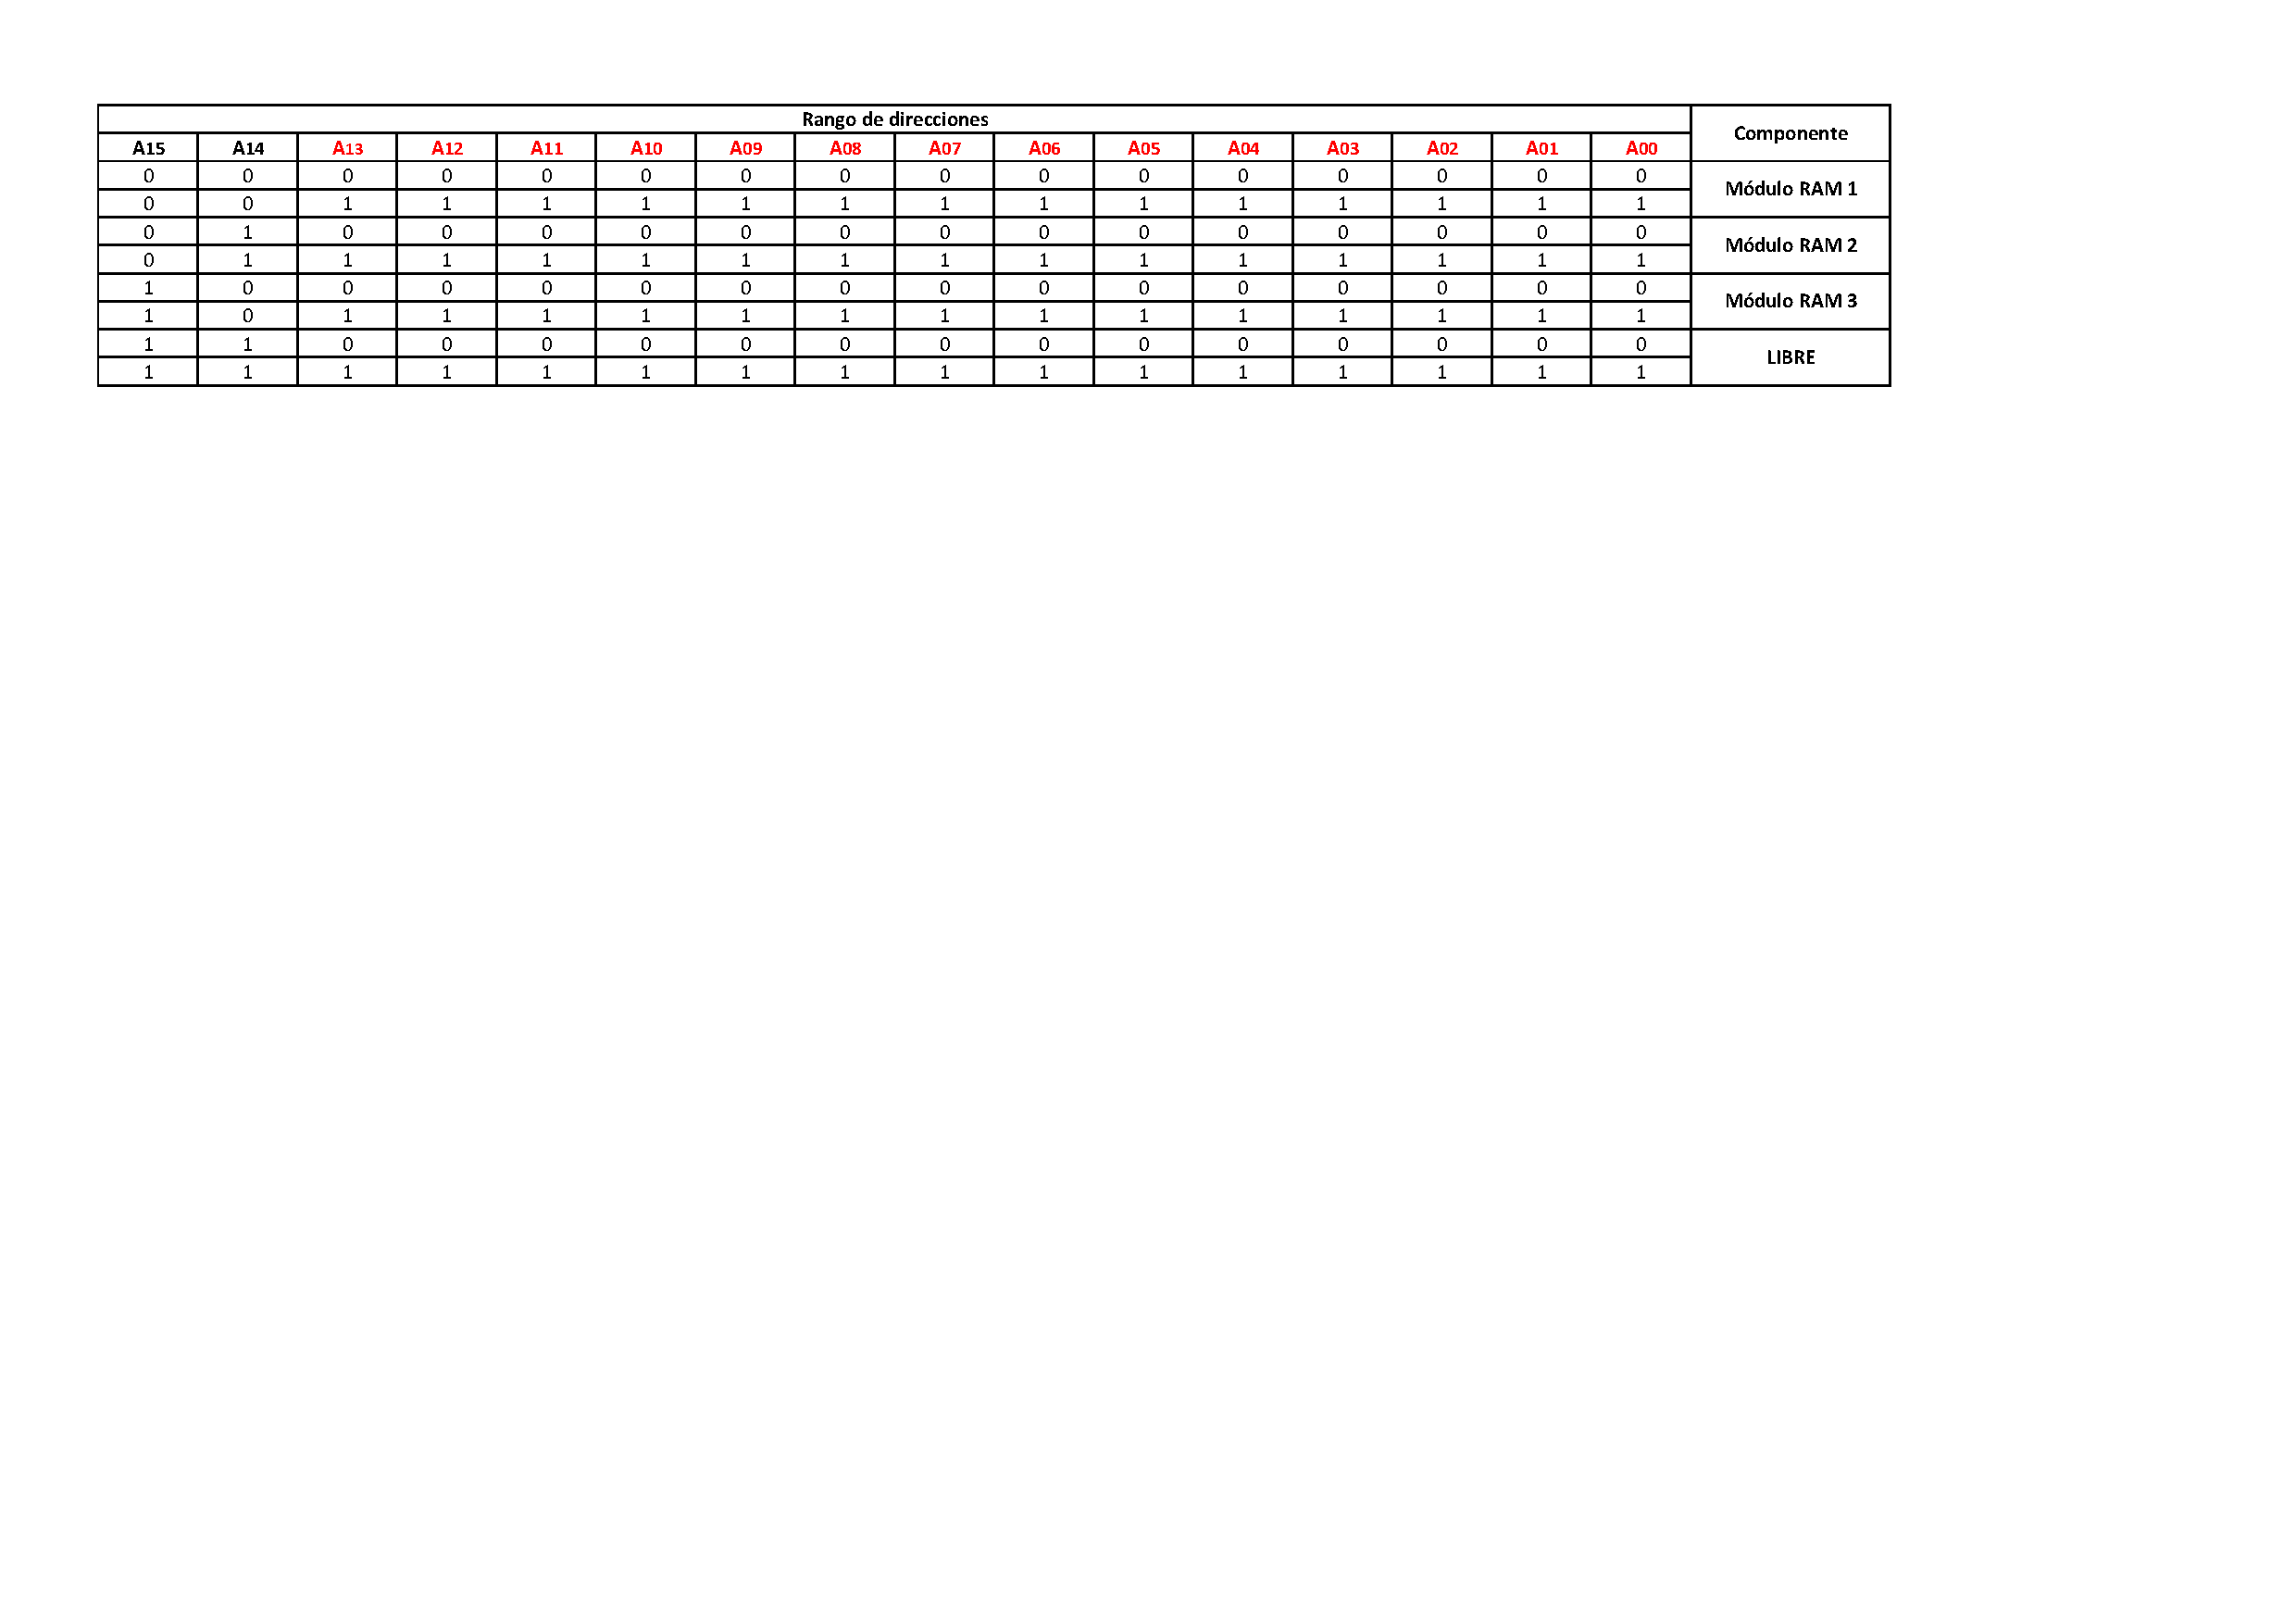
\includegraphics[scale=0.475]{Mapa_memoria_52.pdf}
\end{center}



\end{document}